\let\negmedspace\undefined
\let\negthickspace\undefined
\documentclass[journal]{article}
\usepackage[a5paper, margin=10mm, onecolumn]{geometry}
\usepackage{lmodern} % Ensure lmodern is loaded for pdflatex

\setlength{\headheight}{1cm} % Set the height of the header box
\setlength{\headsep}{0mm}     % Set the distance between the header box and the top of the text

\usepackage{gvv-book}
\usepackage{gvv}
\usepackage{cite}
\usepackage{textcomp}
\usepackage{amsmath,amssymb,amsfonts,amsthm}
\usepackage{algorithmic}
\usepackage{graphicx}
\graphicspath{{./figs/}}
\usepackage{textcomp}
\usepackage{xcolor}
\usepackage{txfonts}
\usepackage{listings}
\usepackage{enumitem}
\usepackage{mathtools}
\usepackage{gensymb}
\usepackage{comment}
\usepackage[breaklinks=true]{hyperref}
\usepackage{tkz-euclide} 
\usepackage{listings}
\usepackage{gvv}                                        
\def\inputGnumericTable{}                                 
\usepackage[latin1]{inputenc}                                
\usepackage{color}                                            
\usepackage{array}                                            
\usepackage{longtable}                                       
\usepackage{calc}                                             
\usepackage{multirow}                                         
\usepackage{hhline}                                           
\usepackage{ifthen}                                           
\usepackage{lscape}
\usepackage{circuitikz}
\tikzstyle{block} = [rectangle, draw, fill=blue!20, 
text width=4em, text centered, rounded corners, minimum height=3em]
\tikzstyle{sum} = [draw, fill=blue!10, circle, minimum size=1cm, node distance=1.5cm]
\tikzstyle{input} = [coordinate]
\tikzstyle{output} = [coordinate]


\begin{document}
	
	\bibliographystyle{IEEEtran}
	\vspace{3cm}
	
\title{2.10.75}
\author{EE25BTECH11047 - RAVULA SHASHANK REDDY}
\maketitle
\hrulefill
\bigskip 

\renewcommand{\thetable}{\theenumi}
\setlength{\intextsep}{10pt}

\textbf{Question:} \\

The points with position vectors $\vec{a}+\vec{b},\;\vec{a}-\vec{b}$ and $\vec{a}+k\vec{b}$ are collinear for all real values of   $k$.Prove

\textbf{Solution:}\\

Given:
\begin{align}
    \vec{P} &= \myvec{\vec{a}&\vec{b}}\myvec{1\\1},\vec{Q}=\myvec{\vec{a}&\vec{b}}\myvec{1\\-1},\vec{R} =\myvec{\vec{a}&\vec{b}}\myvec{1\\k} \\
    \vec{P}-\vec{Q} &=\myvec{\vec{a}&\vec{b}}\myvec{0\\2} \\ 
    \vec{R}-\vec{P} &= \myvec{\vec{a}&\vec{b}}\myvec{0\\k-1}\\[6pt]
    M &= \myvec{ \vec{P}-\vec{Q} & \vec{R}-\vec{P} } 
       = \myvec{ 0 & 0\\2\vec{b} & (k-1)\vec{b} } \\[6pt]
      M& = \vec{b} \myvec{0&0\\2 & k-1}\\
\text{rank}(M) \leq 1.
\end{align}
\begin{center}
Therefore, the two difference vectors are linearly dependent. \\ 

Hence, the points $\vec{P}, \vec{Q}, \vec{R}$ are collinear for all real $k$.
\end{center}

For Example:\\

Take 
\begin{align}
\vec{a}=\myvec{1 \\ 2},\; \vec{b}=\myvec{3 \\ 1}.
\end{align}
For $k=0$:
\begin{align}
\vec{R} = \myvec{1+3(0) \\ 2+0} = \myvec{1 \\ 2}.
\end{align}
For $k=1$:
\begin{align}
\vec{R} = \myvec{1+3(1) \\ 2+1} = \myvec{4 \\ 3}.
\end{align}
For $k=2$:
\begin{align}
\vec{R} = \myvec{1+3(2) \\ 2+2} = \myvec{7 \\ 4}.
\end{align}

So the three points are:
\begin{align}
\vec{Q} &= \myvec{-2 \\ 1}, 
\vec{P} = \myvec{4 \\ 3}, \\
\vec{R} &= \myvec{1 \\ 2}\;(k=0),\; \myvec{4 \\ 3}\;(k=1),\; \myvec{7 \\ 4}\;(k=2).\\
M(k) &= \myvec{\,\vec{P}-\vec{Q} & \vec{R}-\vec{P}\,} 
     = \myvec{6 & 3k-3 \\[4pt] 2 & k-1}.
\end{align}

For $k=0$:
\begin{align}
M(0) = \myvec{6 & -3 \\ 2 & -1}, \quad \text{rank}(M(0))=1.
\end{align}

For $k=1$:
\begin{align}
M(1) = \myvec{6 & 0 \\ 2 & 0}, \quad \text{rank}(M(1))=1.
\end{align}

For $k=2$:
\begin{align}
M(2) = \myvec{6 & 3 \\ 2 & 1}, \quad \text{rank}(M(2))=1.
\end{align}
\begin{figure}
    \centering
    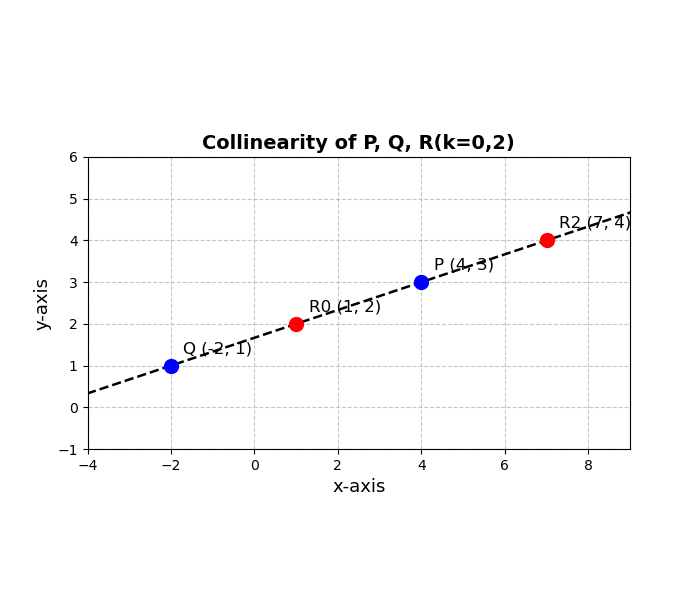
\includegraphics[width=1.0\linewidth]{figs/fig 1.png}
    \caption{Caption}
    \label{fig:placeholder}
\end{figure}
\end{document}